\section{Non-Interactive Proofs of Proofs of Work}

\subsection{Sublinear SPV}
We would like to be able to prove statements like:

\begin{itemize}
  \item We have a valid chain where the last $k$ blocks are the ones we're claiming. This is called a \textbf{suffix proof}.
  \item We have a valid chain where a specific given block is included. This is called an \textbf{infix proof}.
\end{itemize}

Our current best solution, SPV, requires providing the whole chain's block headers as proof. This is obviously linear in the size of the chain.

There have been previous attempts to create proofs smaller in size than SPV proofs~\cite{KLS}, where a scheme for logarithmic proofs was proposed.  This scheme was later proven insecure~\cite{nipopows}.

NIPoPoWs is the first secure construction~\cite{nipopows} for logarithmic proofs.

\subsection{Assumptions}
An assumption NIPoPoWs make is that the difficulty is constant. This is not true for Bitcoin or Bitcoin Cash.

NIPoPoWs also assume each block contains an interlink data structure, which we'll study shortly. Interlinks too don't exist in Bitcoin or Bitcoin Cash.

In the next section we'll look at how we sidestep all those issues.

\subsection{Levels}
At the heart of the primitive lies the separation of blocks into levels. The level of a block is defined as $\textit{level}(B) = \left \lfloor \log(T) - \log(\sf{id}(B)) \right \rfloor$, where $T$ is the constant difficulty of the blockchain. The genesis block is an exception to this rule as $\textit{level}(Gen) = \infty$. We call a block of level $\mu$ a $\mu$-superblock.

Intuitively, the level of a block is the number of leading zeros of the binary representation of the block id when left padded to the length of $T$. An example of this can be seen on Table~\ref{table:level-counting}.

\begin{table}
  \centering
  \begin{tabular}{|c|c|}
    \hline
    $T$ & 1110000 \\
    \hline
    $\sf{id}(B)$ & \underline{000}1000 \\
    \hline
  \end{tabular}
  \caption{Calculating the level of a block by counting the leading zeros (3 in this case).}
  \label{table:level-counting}
\end{table}

Figure~\ref{fig:hierarchy} shows an example the implied blockchain created from the superblocks.

\begin{figure}
  \centering
  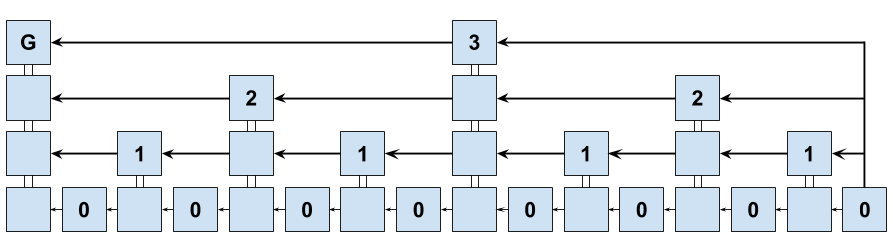
\includegraphics[width=0.9\columnwidth,keepaspectratio]{figures/hierarchical-ledger.png}
  \caption{The hierarchical blockchain.  Higher levels have achieved a lower target (higher difficulty) during mining. All blocks are connected to the genesis block $G$. Source:~\cite{nipopows}}
  \label{fig:hierarchy}
\end{figure}

\subsection{Notation}
The NIPoPoWs paper introduces some notation for talking about blockchains with levels which we'll be using extensively. The notation is widely influenced by Python. Specifically:

\begin{itemize}
  \item $\chain$ denotes a blockchain, with $\chain[0]$ being the genesis block, $\chain[k]$ being the $k$-th first block and $\chain[-k]$ being the $k$-th last block.
  \item $\chain[k:]$ denotes the sub-blockchain starting from the $k$-th block, $\chain[-k:]$ denotes the sub-blockchain starting from the $k$-th last block.
  \item $\chain[:k]$ denotes the sub-blockchain ending before the $k$-th block, $\chain[:-k]$ denotes the sub-blockchain ending before the $k$-th last block.
  \item $\chain[i:j]$ denotes the sub-blockchain starting from the $i$-th block and ending at the $j$-th block. $i$ and $j$ can also be negative numbers similar to above.
  \item $\chain\{B:\}$ denotes the sub-blockchain starting from the block with block id $B$.
  \item $\chain\upchain^\mu$ denotes the sub-blockset of $\chain$ where all blocks are of level $\mu$ or higher.
\end{itemize}

\subsection{Interlink}
Instead of keeping only the hash of the previous block inside the block header, for every superblock level we keep a pointer to the most recent superblock of that level. The structure containing these pointers is called the interlink. Bitcoin does not support such a structure in the block header but we will study how to sidestep this issue by velvet forking in a few sections.

\begin{table}
  \centering
  \begin{tabular}{|c|c|}
    \hline
    Level & Block \\
    \hline
    $0$ & $C[-2]$ \\
    $1$ & $C[-2]$ \\
    $2$ & $C[-4]$ \\
    $3$ & $C[-8]$ \\
    $\infty$ & $C[0]$ \\
    \hline
  \end{tabular}
  \caption{Interlink of $C[-1]$ from Figure~\ref{fig:hierarchy}}
  \label{table:interlink-example}
\end{table}

It's important to note that the interlink can be encoded as a series of block ids, starting from $0$ up to $\infty$. It can also be compressed by using this series as the leafs of a Merkle tree and taking the Merkle tree root.

\subsection{Suffix Proofs}
Suffix proofs are parameterized by $k$ and $m$. $k$ refers to the number of blocks that need to bury a block for it to be considered stable.

A suffix proof of a chain $\chain$ is constituted of two chains, $\pi$ and $\chi$. The final proof is the concatenation of those two chains $\pi \chi$. $\chi$ always refers to the chain of unstable blocks and is evaluated as $\chi = \chain[-k:]$.

The process for constructing $\pi$ is a little more convoluted. First we have to find the first level $\mu$ where $|\chain\upchain^\mu| \ge m$. We call this level $max\mu$. For this level we take all its blocks except for the last $m$: $\pi_{max\mu} = \chain\upchain^\mu[:-m]$. Then for every level $\mu$ from $max\mu - 1$ to $0$, we take blocks $\pi_\mu = \chain\upchain^\mu [:-m]\{\chain\upchain^{\mu+1}[-m]:\}$.

$\pi$ is then evaluated as the concatenation of all those chains starting from the oldest block:

$$ \pi = \pi_{max\mu} || \pi_{max\mu-1} || \ldots || \pi_0 $$

\begin{figure}
  \centering
  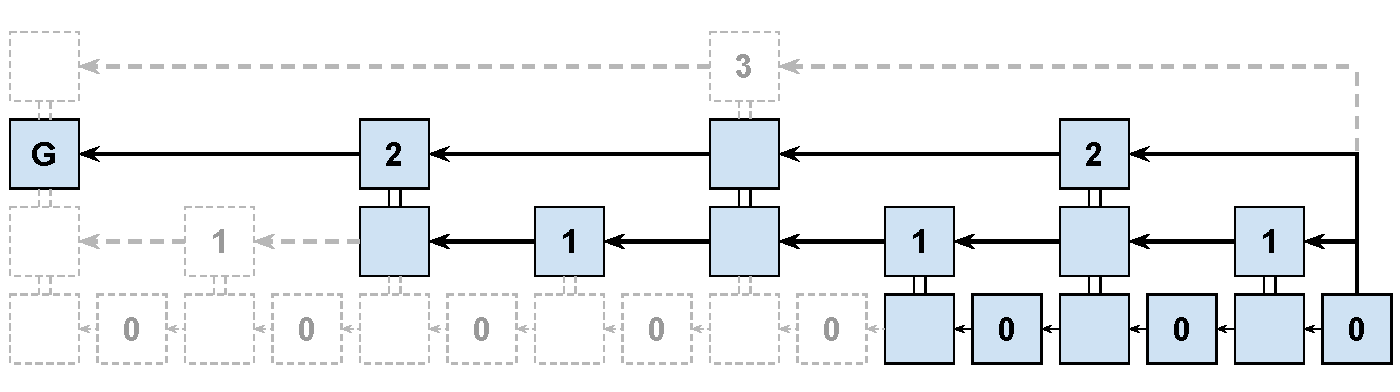
\includegraphics[width=0.9\columnwidth,keepaspectratio]{figures/non-interactive-popow.pdf}
  \caption{Construction of $\pi$ of a suffix proof. $m=3$  Source:~\cite{nipopows}}
  \label{fig:suffix-proof}
\end{figure}

It's important to notice that the chain provided to the verifier is an actual chain: one can start at the end and traverse it until the genesis block by utilizing the interlink of each block, similar to how they would do that on a conventional blockchain by using each block's $\sf previd$.

\subsection{Infix Proofs}
For the verifier to be able to determine a predicate on one or more blocks ($\chain' \subseteq \chain$) of our chain, we have to make sure we include them in a proof. A suffix proof is not guaranteed to include all blocks of interest in $\chain'$. In order to include these we have to make sure they are linked to the proof, e.g. that the proof chain is a traversable. To this end, let's assume some arbitrary block $B \in \chain'$. Let's also assume an existing suffix proof $\pi\chi$. We find blocks $E'$ and $E$ on the suffix proof, such that:

\begin{itemize}
  \item $E$ is the next block after $E'$ on the proof
  \item $B$ comes before $E$ on $\chain$
  \item $B$ comes after $E'$ on $\chain$
\end{itemize}

An example of such a triplet of blocks satisfying those conditions can be seen on Figure~\ref{fig:infix-proof}.

\begin{figure}
  \centering
  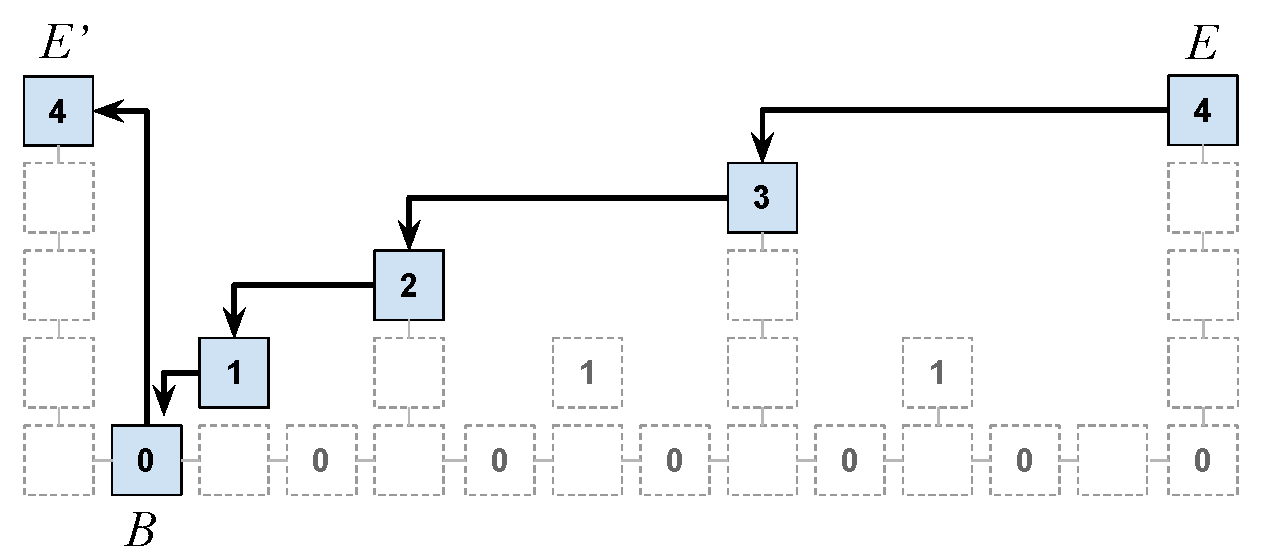
\includegraphics[width=0.9\columnwidth,keepaspectratio]{figures/infix.pdf}
  \caption{Construction of an infix proof.  Source:~\cite{nipopows}}
  \label{fig:infix-proof}
\end{figure}

We then perform a procedure called $\sf followDown$ in order to figure out which blocks need to be added to the proof in order to link $E$ to $B$. $\sf followDown$ includes blocks on intermediate levels until $B$ is reached. The full algorithm can be seen on Algorithm~\ref{alg.nipopow-infix-follow}.

\begin{algorithm}[H]
    \caption{\label{alg.nipopow-infix-follow}The \textsf{followDown} function
    which produces the necessary blocks to connect a superblock $E$ to a
    preceeding regular block $B$.  Source:~\cite{nipopows}}
    \begin{algorithmic}[1]
        \Function{\sf followDown}{$E$, $B$, \textsf{height}} %, realLink, blockById}
            \State{$aux \gets \emptyset$; $\mu \gets \textit{level}(E)$}
            \While{$E \neq B$}
                \Let{B'}{\textsf{blockById}[E\text{.interlink}[\mu]]}
                \If{$\textsf{height}[B'] < \textsf{height}[B]$}
                    \Let{\mu}{\mu - 1}
                \Else
                    \Let{aux}{aux \cup \{E\}}
                    \Let{E}{B'}
                \EndIf
            \EndWhile
            \State\Return{$aux$}
        \EndFunction
    \vskip8pt
    \end{algorithmic}
\end{algorithm}


Augmenting the original suffix proof with the new blocks provided by $\sf followDown$ on all our blocks of interest $B \in \chain'$ gives us our final infix proof. Note that as was the case with our suffix proofs, the infix proof is traversable.

\subsection{Proof Verification}
\subsection{Velvet Forks}
Velvet forks~\cite{nipopows,velvet} describe a formalization of adding arbitrary data inside blocks in order to allow potential applications without sacrificing the backwards compatibility of the blockchain.

Miners who are willing to contribute to the fork can add data of interest in the form of coinbase transaction data. 

Backwards compatibility is achieved by not changing the consensus rules, meaning that set of acceptable blocks does not change. So any block that was acceptable remains acceptable even if it does not contain any data concerning the fork, or if it contains invalid data.

\subsection{User-Activated Velvet Forks}
In case miners aren't interested in including such data, users can also create such a fork by making a kind of transaction called velvet transaction. In a velvet transaction a user includes any data of interest in unspendable transaction outputs (like OP\_RETURN).

For the consumer of such data, the only difference is that they have to look inside the whole block to find it, not only inside the coinbase data.

Such forks come at the cost of making such transactions, because the user who makes the fork needs to pay transaction fees every time they wish to add data to the blockchain.

For our application, we implemented a User-Activated Velvet Fork in order to add the interlink data structure to Bitcoin Cash blocks. Since Bitcoin Cash has very low fees, a projection of running such a fork comes at around 10€/month.
